\section{Logo Trends}
\label{app:logotrends}

\subsection{2012}

\begin{figure}[h!]
  \centering
  \begin{subfigure}{.45\textwidth}
    \centering
    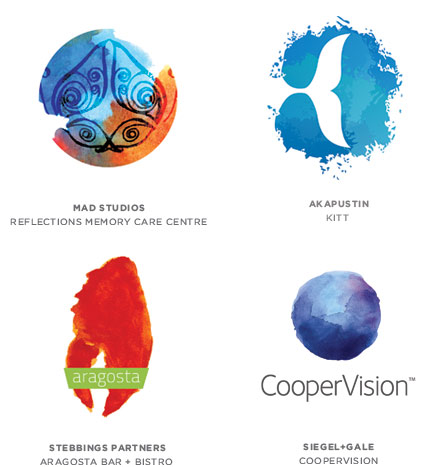
\includegraphics[width=\linewidth]{images/supplement/logolounge/2012/Akvarel'}
    \caption{Акварель}
    \label{fig:logolounge:2012:akvarel'}
  \end{subfigure}
  \hfill
  \centering
  \begin{subfigure}{.45\textwidth}
    \centering
    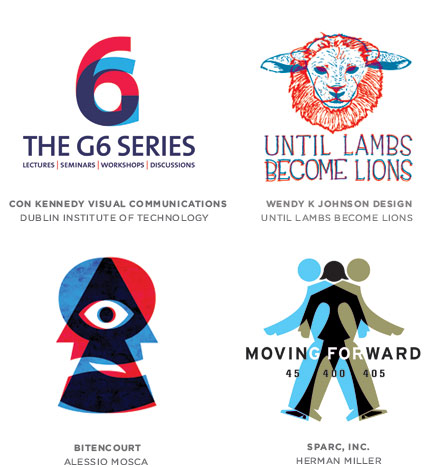
\includegraphics[width=\linewidth]{images/supplement/logolounge/2012/Anaglifi}
    \caption{Анаглифы}
    \label{fig:logolounge:2012:anaglifi}
  \end{subfigure}
  \vfill
  \centering
  \begin{subfigure}{.45\textwidth}
    \centering
    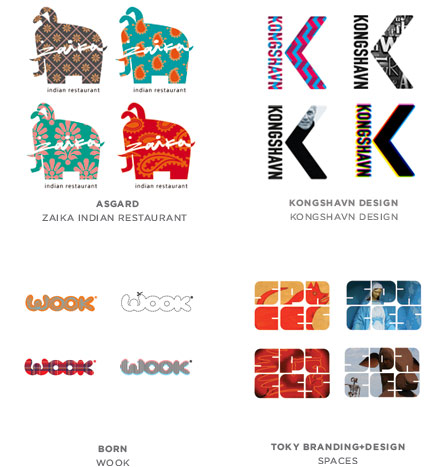
\includegraphics[width=\linewidth]{images/supplement/logolounge/2012/Bratskie-serii.jpeg}
    \caption{Братские серии}
    \label{fig:logolounge:2012:bratskie-serii}
  \end{subfigure}
  \hfill
  \centering
  \begin{subfigure}{.45\textwidth}
    \centering
    
\includegraphics[width=\linewidth]{images/supplement/logolounge/2012/Chipsi}
    \caption{Чипсы}
    \label{fig:logolounge:2012:chipsi}
  \end{subfigure}
\end{figure}

\begin{figure}[h!]
  \ContinuedFloat
  \centering
  \begin{subfigure}{.45\textwidth}
    \centering
    
\includegraphics[width=\linewidth]{images/supplement/logolounge/2012/Klasteri-ikonok.jpeg}
    \caption{Кластеры иконок}
    \label{fig:logolounge:2012:klasteri-ikonok}
  \end{subfigure}
  \hfill
  \centering
  \begin{subfigure}{.45\textwidth}
    \centering
    
\includegraphics[width=\linewidth]{images/supplement/logolounge/2012/Kojura}
    \caption{Кожура}
    \label{fig:logolounge:2012:kojura}
  \end{subfigure}

  \vfill

  \centering
  \begin{subfigure}{.45\textwidth}
    \centering
    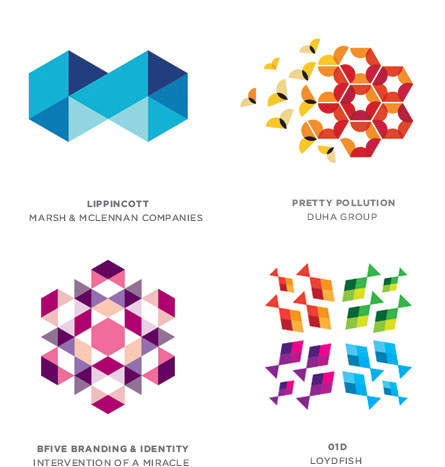
\includegraphics[width=\linewidth]{images/supplement/logolounge/2012/Mozaiki}
    \caption{Мозаики}
    \label{fig:logolounge:2012:mozaiki}
  \end{subfigure}
  \hfill
  \centering
  \begin{subfigure}{.45\textwidth}
    \centering
    
\includegraphics[width=\linewidth]{images/supplement/logolounge/2012/Prilojeniya}
    \caption{Приложения}
    \label{fig:logolounge:2012:prilojeniya}
  \end{subfigure}
\end{figure}

\begin{figure}[h!]
  \ContinuedFloat
  \centering
  \begin{subfigure}{.45\textwidth}
    \centering
    
\includegraphics[width=\linewidth]{images/supplement/logolounge/2012/Prozrachnie-zepochki.jpeg}
    \caption{Прозраченые цепочки}
    \label{fig:logolounge:2012:prozrachnie-zerpochki}
  \end{subfigure}
  \hfill
  \centering
  \begin{subfigure}{.45\textwidth}
    \centering
    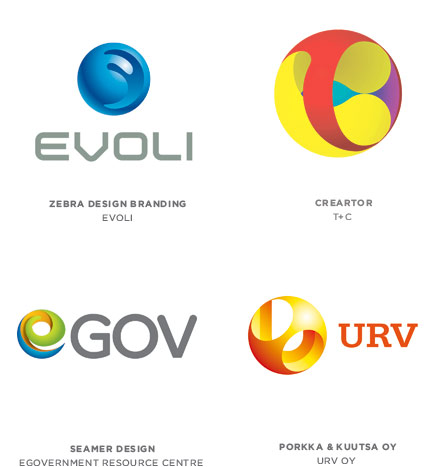
\includegraphics[width=\linewidth]{images/supplement/logolounge/2012/Rezba-v-sferah.jpeg}
    \caption{Резьба в сферах}
    \label{fig:logolounge:2012:rezba-v-sferah}
  \end{subfigure}

  \vfill

  \centering
  \begin{subfigure}{.45\textwidth}
    \centering
    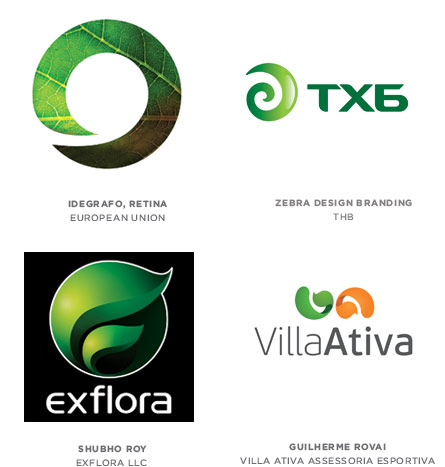
\includegraphics[width=\linewidth]{images/supplement/logolounge/2012/Rostki}
    \caption{Ростки}
    \label{fig:logolounge:2012:rostki}
  \end{subfigure}
  \hfill
  \centering
  \begin{subfigure}{.45\textwidth}
    \centering
    \includegraphics[width=\linewidth]{images/supplement/logolounge/2012/tkan'}
    \caption{Ткань}
    \label{fig:logolounge:2012:tkan'}
  \end{subfigure}
\end{figure}

\begin{figure}[h!]
  \ContinuedFloat
  \centering
  \begin{subfigure}{.45\textwidth}
    \centering
    
\includegraphics[width=\linewidth]{images/supplement/logolounge/2012/Viborochnaya-rexkost'.jpeg}
    \caption{Выборочная резкость}
    \label{fig:logolounge:2012:viborichnaya-rexkost'}
  \end{subfigure}
  \hfill
  \centering
  \begin{subfigure}{.45\textwidth}
    \centering
    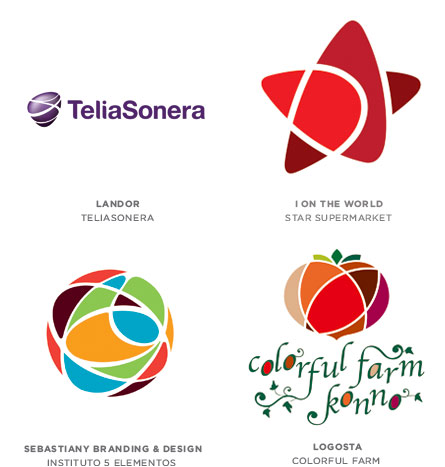
\includegraphics[width=\linewidth]{images/supplement/logolounge/2012/Zavitushki}
    \caption{Завитушки}
    \label{fig:logolounge:2012:zavitushki}
  \end{subfigure}

  \vfill

  \centering
  \begin{subfigure}{.45\textwidth}
    \centering
    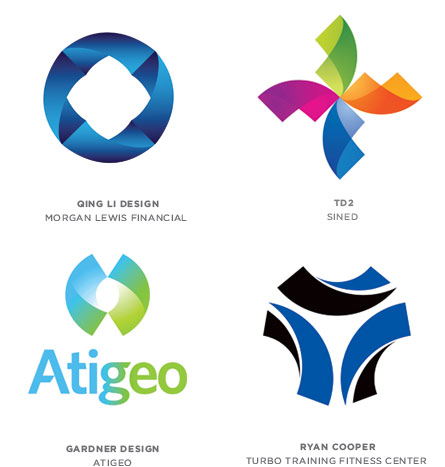
\includegraphics[width=\linewidth]{images/supplement/logolounge/2012/Zakruxhennie-dugi.jpeg}
    \caption{Закругленные дуги}
    \label{fig:logolounge:2012:zakruxhennie-dugi}
  \end{subfigure}
\end{figure}


\FloatBarrier
\subsection{2013}

\begin{figure}[h!]
  \centering
  \begin{subfigure}{.45\textwidth}
    \centering
    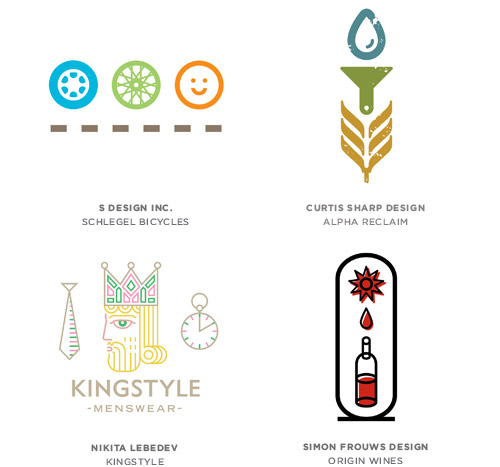
\includegraphics[width=\linewidth]{images/supplement/logolounge/2013/Formula}
    \caption{Формула}
    \label{fig:logolounge:2013:formula}
  \end{subfigure}
  \hfill
  \centering
  \begin{subfigure}{.45\textwidth}
    \centering
    
\includegraphics[width=\linewidth]{images/supplement/logolounge/2013/Kresti}
    \caption{Кресты}
    \label{fig:logolounge:2013:kresti}
  \end{subfigure}
  \vfill
  \centering
  \begin{subfigure}{.45\textwidth}
    \centering
    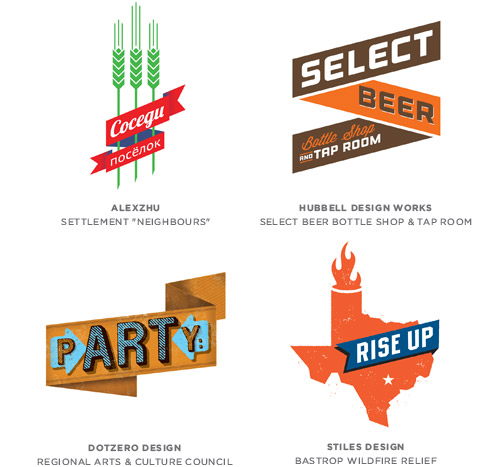
\includegraphics[width=\linewidth]{images/supplement/logolounge/2013/Lenti}
    \caption{Ленты}
    \label{fig:logolounge:2013:lenti}
  \end{subfigure}
  \hfill
  \centering
  \begin{subfigure}{.45\textwidth}
    \centering
    
\includegraphics[width=\linewidth]{images/supplement/logolounge/2013/Membrana}
    \caption{Мембрана}
    \label{fig:logolounge:2013:membrana}
  \end{subfigure}
\end{figure}

\begin{figure}[h!]
  \ContinuedFloat
  \centering
  \begin{subfigure}{.45\textwidth}
    \centering
    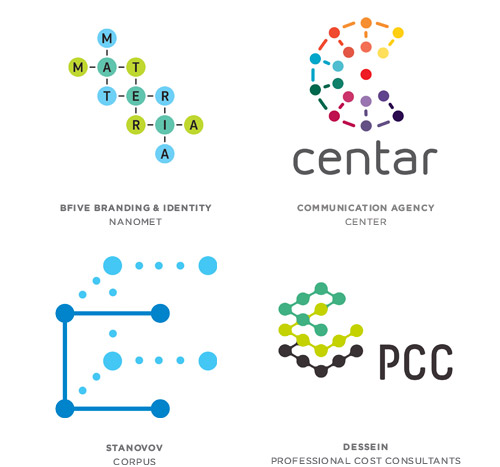
\includegraphics[width=\linewidth]{images/supplement/logolounge/2013/Molekuli}
    \caption{Молекулы}
    \label{fig:logolounge:2013:moleculi}
  \end{subfigure}
  \hfill
  \centering
  \begin{subfigure}{.45\textwidth}
    \centering
    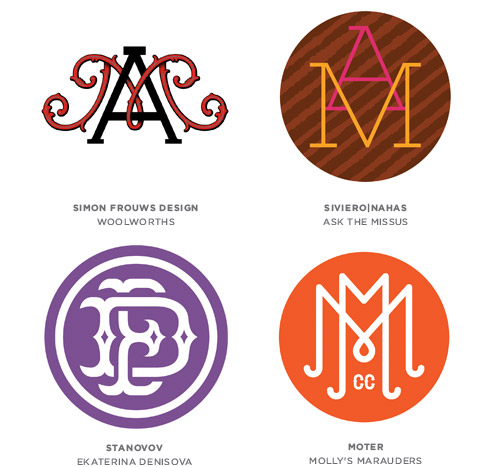
\includegraphics[width=\linewidth]{images/supplement/logolounge/2013/Monogrammi}
    \caption{Монограммы}
    \label{fig:logolounge:2013:Monogrammi}
  \end{subfigure}

  \vfill

  \centering
  \begin{subfigure}{.45\textwidth}
    \centering
    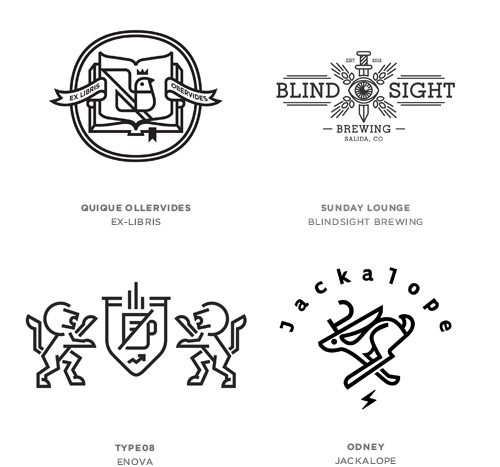
\includegraphics[width=\linewidth]{images/supplement/logolounge/2013/Monoshirinnaya-liniya}
    \caption{Моноширинная линия}
    \label{fig:logolounge:2013:monoshirinnaya-liniya}
  \end{subfigure}
  \hfill
  \centering
  \begin{subfigure}{.45\textwidth}
    \centering
    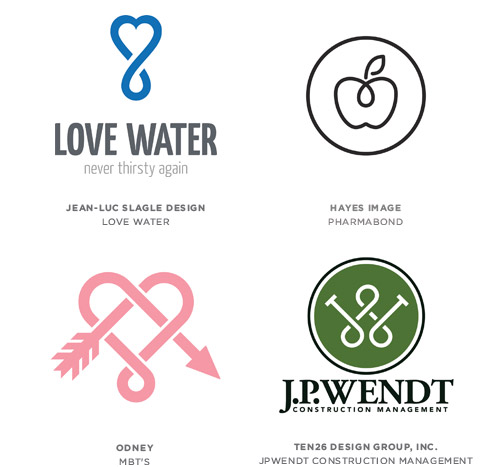
\includegraphics[width=\linewidth]{images/supplement/logolounge/2013/Petlya}
    \caption{Петля}
    \label{fig:logolounge:2013:petlya}
  \end{subfigure}
\end{figure}

\begin{figure}[h!]
  \ContinuedFloat
  \centering
  \begin{subfigure}{.45\textwidth}
    \centering
    
\includegraphics[width=\linewidth]{images/supplement/logolounge/2013/Skobki}
    \caption{Скобки}
    \label{fig:logolounge:2013:skobki}
  \end{subfigure}
  \hfill
  \centering
  \begin{subfigure}{.45\textwidth}
    \centering
    
\includegraphics[width=\linewidth]{images/supplement/logolounge/2013/Skveomorfism}
    \caption{Сквеоморфизм}
    \label{fig:logolounge:2013:skveomorfism}
  \end{subfigure}

  \vfill

  \centering
  \begin{subfigure}{.45\textwidth}
    \centering
    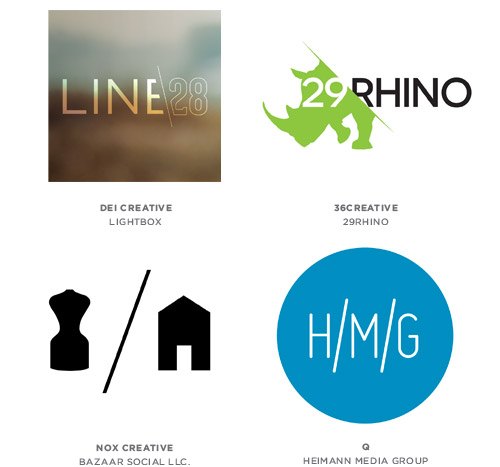
\includegraphics[width=\linewidth]{images/supplement/logolounge/2013/Slesh}
    \caption{Слэш}
    \label{fig:logolounge:2013:slesh}
  \end{subfigure}
  \hfill
  \centering
  \begin{subfigure}{.45\textwidth}
    \centering
    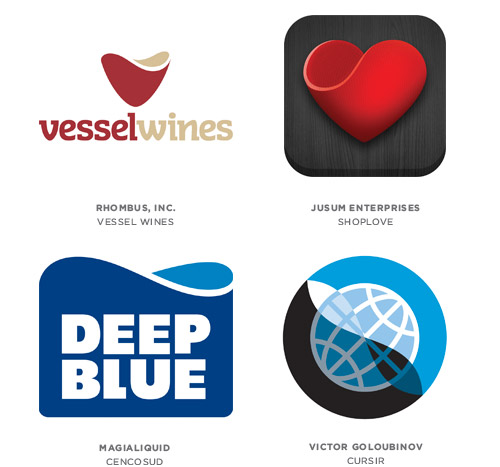
\includegraphics[width=\linewidth]{images/supplement/logolounge/2013/Volni}
    \caption{Волны}
    \label{fig:logolounge:2013:volni}
  \end{subfigure}
\end{figure}

\begin{figure}[h!]
  \ContinuedFloat
  \centering
  \begin{subfigure}{.45\textwidth}
    \centering
    
\includegraphics[width=\linewidth]{images/supplement/logolounge/2013/Vpisannij-tekst}
    \caption{Вписанный текст}
    \label{fig:logolounge:2013:vpisannij-tekst}
  \end{subfigure}
  \hfill
  \centering
  \begin{subfigure}{.45\textwidth}
    \centering
    
\includegraphics[width=\linewidth]{images/supplement/logolounge/2013/Znachki}
    \caption{Значки}
    \label{fig:logolounge:2013:znachki}
  \end{subfigure}

  \vfill

  \centering
  \begin{subfigure}{.45\textwidth}
    \centering
    
\includegraphics[width=\linewidth]{images/supplement/logolounge/2013/Znachok-zdes}
    \caption{Значок <<Здесь>>}
    \label{fig:logolounge:2013:znachok-zdes}
  \end{subfigure}
\end{figure}
